\begin{problem}{七星珠}{七星珠.in}{七星珠.out}{1 second}


故事背景:《鲁滨逊漂流记》是Michael Robison执导,菲利普·温彻斯特、安娜·沃尔顿等主演的电视剧。该剧描述探险家鲁滨逊在一次航行中船只失事,流落到一个杳无人烟的荒岛长达28年时间,完全与世隔绝的故事。---来自百度百科\\
问题描述:由于最近热身赛表现不佳,小本同学被Mr Zhou流放到了一个荒无人烟的岛上,岛上没有什么娱乐设施,与之相伴的只有各种各样奇形怪状的石头,现在Mr Zhou给小本同学出了一道这样的数学题:已知岛上一共有各种不同体积的石头$N$种,每种石头$i$都有自己的体积$v_i$和数量$w_i$,现在Mr Zhou给出一个正整数$T$,要求小本计算一下,如何组合可以满足组成$T$体积的石头数量最多。如果小本能解答出这个问题,Mr Zhou将安排他离开这个荒岛,如果不能,那只能在岛上度过余生了$\^{} \_ \^{}$。为了简化期间,小本只要计算出组成$T$体积的最多石头的数量即可,如果无法组合出$T$体积,则答案为$0$。
\begin{center}
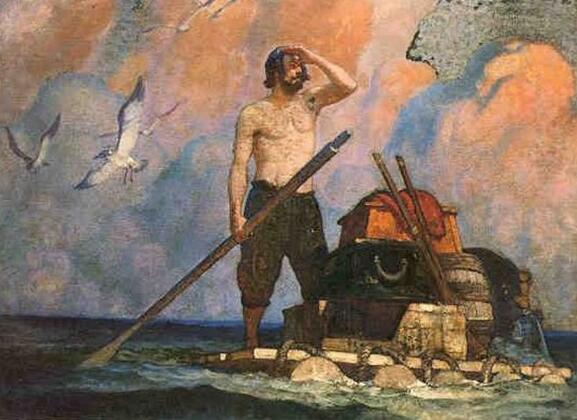
\includegraphics[width=0.5\textwidth]{pics/G.jpg}
\end{center}
\InputFile
第一行输入正整数$N\ (1\le N\le 1000)$和$T\ (1\le T\le 10^6)$,表示岛上石头的种类和所要组合出的体积。

接下来$N$行每行输入两个正整数$v_i(1\le v_i\le 10^5)$和$w_i(1\le w_i\le 1000)$表示$i$号石头的体积和数量。
\OutputFile
输出组合成$T$的最大石头数量,无法组成$T$则输出$0$。
\Example
\begin{example}
\exmp{
5 8
1 2
2 3
1 2
3 3
4 2
}{
5
}%
\end{example}
\end{problem}